
\chapter{Simulator Interface}

\section{Main Window}

The main window consists of a menu, a status bar, a frequency selection combobox, an on/off button to trigger debugging, some board-specific controls and the part of the board interface itself.

In the title of the window is shown the name of the simulator PICSimLab, followed by the board and the microcontroller in use.


\begin{figure}[H]
\center
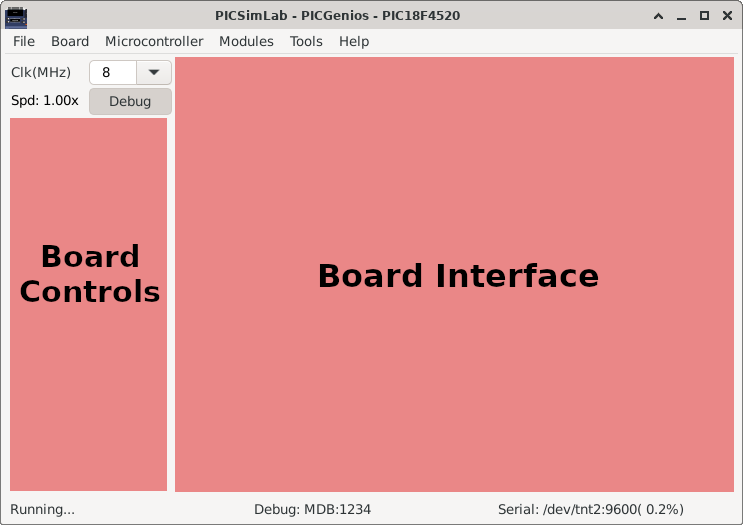
\includegraphics[width=0.99\textwidth]{img/int.png} 
\end{figure} 

The frequency selection combobox directly changes the working speed of the microcontroller.
The ``Spd'' label show the ratio between simulation speed and real time. when the ``Spd'' label goes red indicates that the computer is not being able to run the program in real time for the selected clock. 
In this case the simulation may present some difference than expected and the CPU load will be increased.

The on/off button to enable debugging is used to enable debugging support, when active simulation load is increased.

The menus and their functions are listed below:
\begin{itemize}
\item File
\begin{itemize}
\item Load Hex - Load .hex files
\item Reload Last - Reload the last used .hex file
\item Save Hex - Save memory in a .hex file
\item Configure - Open the configuration windows
\item Save Workspace - Saves all current workspace settings to a .pzw file
\item Load Workspace - Loads saved settings from a .pzw file
\item Exit
\end{itemize}
\item Board
\begin{itemize}
\item Arduino Uno - Choose board Arduino Uno
\item Breadboard - Choose board Breadboard
\item Franzininho - Choose board Franzininho
\item K16F - Choose board K16F
\item McLab1 - Choose board McLab1
\item McLab2 - Choose board McLab2
\item PICGenios - Choose board PICGenios
\item PQDB - Choose board PQDB
\end{itemize}
\item Microcontroller
\begin{itemize}
 \item xxxxx - Selects the microcontroller to be used (depends on the selected board)
\end{itemize}
\item Modules
\begin{itemize}
\item Oscilloscope - Open the oscilloscope window
\item Spare parts - Open the spare parts window
\end{itemize}
\item Tools 
\begin{itemize}
 \item Serial Terminal - Open the serial terminal \hyperlink{def:sterm}{Cutecom}
 \item Serial Remote Tank - Open the \hyperlink{def:srtank}{remote tank simulator}
 \item Esp8266 Modem Simulator -  Open the \hyperlink{def:espmsim}{Esp8266 Modem Simulator}
 \item Arduino Bootloader - Load microcontroller with \hyperlink{def:aboot}{Arduino serial bootloader} 
 \item MPLABX Debugger Plugin - Open the web page to download the \hyperlink{def:mpdebug}{MPLABX Debugger Plugin} 
 \item Pin Viewer - Open the \hyperlink{def:pinv}{Pin Viewer} 
\end{itemize}
\item Help 
\begin{itemize}
 \item Contents - Open the Help window
 \item Board - Open the Board Help window
 \item Examples - Load the examples
 \item About Board - Show message about author and version of board
 \item About PICSimLab - Show message about author and version of PICSimLab
\end{itemize}
\end{itemize}


\begin{figure}[H]
\center
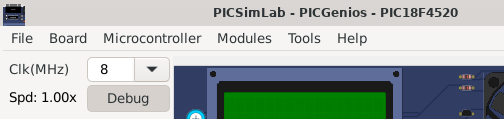
\includegraphics[width=0.85\textwidth]{img/int1.png} 
\end{figure} 

The first part of the status bar shows the state of the simulation, in the middle part the status of the debug support and in the last part the name of the serial port used, its default speed and the error in relation to the real speed configured in the microcontroller.

\begin{figure}[H]
\center
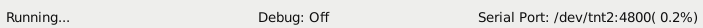
\includegraphics[width=0.85\textwidth]{img/int2.png} 
\end{figure} 


\section{Interaction with the Board}

On the interface area of the board it is possible to interact in some ways:

\begin{itemize}
 \item Click in ICSP connector to load an .hex file.
 \item Click in PWR button to ON/OFF the emulator..
 \item The buttons can be activated through mouse or keys 1, 2, 3 e 4.
 \item Click and drag in potentiometers to change their values.
 \item Click on EEPROM memory to view its contents.
\end{itemize}


\section{Command Line}

PICSimLab supports two command lines format:

One for load a PICSimLab Workspace file (.pzw) 
\begin{minted}[baselinestretch=1.2,fontsize=\footnotesize,bgcolor=colorbash]{bash}
  picsimlab file.pzw
\end{minted}

And other for load .hex files
\begin{minted}[baselinestretch=1.2,fontsize=\footnotesize,bgcolor=colorbash]{bash}
  picsimlab boardname microcontroller [file.hex] [file.pcf]
\end{minted}


\section{Remote Control Interface}\hypertarget{def:rcontrol}{}

The remote control interface allows other programs to control the PICSimLab simulation
through a TCP/IP socket using text formatted commands. 

The PICSimLab remote control interface supports TCP connections using telnet or nc (netcat).

The default port is 5000 and can be changed in configuration windows. 

The 'rlwrap' command can be used for best command edition support in telnet or nc:
\begin{minted}[baselinestretch=1.2,fontsize=\footnotesize,bgcolor=colorbash]{bash}
 rlwrap nc 127.0.0.1 5000
\end{minted}
  
The supported commands can be shown using the ``help'' command:  
\begin{minted}[baselinestretch=1.2,fontsize=\footnotesize,bgcolor=colorbash]{bash}
 help
List of supported commands:
  dumpe [a] [s]- dump internal EEPROM memory
  dumpf [a] [s]- dump Flash memory
  dumpr [a] [s]- dump RAM memory
  exit         - shutdown PICSimLab
  get ob       - get object value
  help         - show this message
  info         - show actual setup info and objects
  loadhex file - load hex file (use full path)  
  pins         - show pins directions and values
  pinsl        - show pins formated info
  quit         - exit remote control interface
  reset        - reset the board
  set ob vl    - set object with value
  sim [cmd]    - show simulation status or execute cmd start/stop
  sync         - wait to syncronize with timer event
  version      - show PICSimLab version
Ok
\end{minted}
  

The ``info'' command show all available "objects" and values:
\begin{minted}[baselinestretch=1.2,fontsize=\footnotesize,bgcolor=colorbash]{bash}
info
Board:     Arduino Uno
Processor: atmega328p
Frequency:   16000000 Hz
Use Spare: 1
    board.out[00] LD_L= 254
  part[00]: LEDs
    part[00].out[08] LD_1= 254
    part[00].out[09] LD_2= 30
    part[00].out[10] LD_3= 254
    part[00].out[11] LD_4= 254
    part[00].out[12] LD_5 254
    part[00].out[13] LD_6= 254
    part[00].out[14] LD_7= 254
  part[01]: Buzzer
    part[01].out[02] LD_1= 140
  part[02]: Push buttons
    part[02].in[00] PB_1= 1
    part[02].in[01] PB_2= 0
    part[02].in[02] PB_3= 1
    part[02].in[03] PB_4= 1
    part[02].in[04] PB_5= 1
    part[02].in[05] PB_6= 1
    part[02].in[06] PB_7= 1
    part[02].in[07] PB_8= 1
Ok
\end{minted}

The ``pins'' command show all pins directions and digital values:
\begin{minted}[baselinestretch=1.2,fontsize=\footnotesize,bgcolor=colorbash]{bash}
pins
  pin[01] ( PC6/RST) < 0                 pin[15] (  PB1/~9) > 0 
  pin[02] (   PD0/0) < 1                 pin[16] ( PB2/~10) > 0 
  pin[03] (   PD1/1) < 1                 pin[17] ( PB3/~11) > 0 
  pin[04] (   PD2/2) < 1                 pin[18] (  PB4/12) < 0 
  pin[05] (  PD3/~3) > 0                 pin[19] (  PB5/13) > 0 
  pin[06] (   PD4/4) < 1                 pin[20] (     +5V) < 1 
  pin[07] (     +5V) < 1                 pin[21] (    AREF) < 0 
  pin[08] (     GND) < 0                 pin[22] (     GND) < 0 
  pin[09] (  PB6/X1) < 0                 pin[23] (  PC0/A0) < 0 
  pin[10] (  PB7/X2) < 0                 pin[24] (  PC1/A1) < 0 
  pin[11] (  PD5/~5) < 1                 pin[25] (  PC2/A2) < 0 
  pin[12] (  PD6/~6) < 1                 pin[26] (  PC3/A3) < 0 
  pin[13] (   PD7/7) < 1                 pin[27] (  PC4/A4) > 0 
  pin[14] (   PB0/8) > 0                 pin[28] (  PC5/A5) > 0 
Ok
\end{minted}

The ``pinsl'' command show all pins info in text formatted output:
\begin{minted}[baselinestretch=1.2,fontsize=\footnotesize,bgcolor=colorbash]{bash}
pinsl
28 pins [atmega328p]:
  pin[01] D I 0 000 0.000 "PC6/RST " 
  pin[02] D I 1 200 0.000 "PD0/0   " 
  pin[03] D I 1 200 0.000 "PD1/1   " 
  pin[04] D I 1 200 0.000 "PD2/2   " 
  pin[05] D O 0 007 0.000 "PD3/~3  " 
  pin[06] D I 1 200 0.000 "PD4/4   " 
  pin[07] P I 1 200 0.000 "+5V     " 
  pin[08] P I 0 000 0.000 "GND     " 
  pin[09] D I 0 000 0.000 "PB6/X1  " 
  pin[10] D I 0 000 0.000 "PB7/X2  " 
  pin[11] D I 1 200 0.000 "PD5/~5  " 
  pin[12] D I 1 200 0.000 "PD6/~6  " 
  pin[13] D I 1 200 0.000 "PD7/7   " 
  pin[14] D O 0 000 0.000 "PB0/8   " 
  pin[15] D O 0 000 0.000 "PB1/~9  " 
  pin[16] D O 0 000 0.000 "PB2/~10 " 
  pin[17] D O 0 006 0.000 "PB3/~11 " 
  pin[18] D I 0 000 0.000 "PB4/12  " 
  pin[19] D O 0 000 0.000 "PB5/13  " 
  pin[20] P I 1 200 0.000 "+5V     " 
  pin[21] R I 0 000 0.000 "AREF    " 
  pin[22] P I 0 000 0.000 "GND     " 
  pin[23] A I 0 000 0.875 "PC0/A0  " 
  pin[24] A I 0 000 1.925 "PC1/A1  " 
  pin[25] A I 0 000 2.700 "PC2/A2  " 
  pin[26] A I 0 000 4.275 "PC3/A3  " 
  pin[27] D O 1 179 0.000 "PC4/A4  " 
  pin[28] D O 1 186 0.000 "PC5/A5  " 
Ok
\end{minted}


You can view one input/output state using the ``get'' command:
\begin{minted}[baselinestretch=1.2,fontsize=\footnotesize,bgcolor=colorbash]{bash}
get board.out[00]

get part[02].in[01]
\end{minted}

Its possible use the ``get'' command to view individual pins state:
\begin{minted}[baselinestretch=1.2,fontsize=\footnotesize,bgcolor=colorbash]{bash}
#digital state
get pin[19]
pin[19]= 0 
Ok

#digital mean value (0-200)
get pinm[19]
pin[18]= 100 
Ok

#analog state
get apin[25]
apin[25]= 2.700
Ok

#all info
get pinl[13]
pin[13] D I 1 200 0.000 "PD7/7   "
Ok
\end{minted}



And set value of one input using the ``set'' command:
\begin{minted}[baselinestretch=1.2,fontsize=\footnotesize,bgcolor=colorbash]{bash}
set part[02].in[01]  0
set part[02].in[01]  1
\end{minted}

Or set value of one pin using the ``set'' command:
\begin{minted}[baselinestretch=1.2,fontsize=\footnotesize,bgcolor=colorbash]{bash}
#digital
set pin[10]  2

#analog
set apin[20] 2.345
\end{minted}



For windows users \href{https://www.putty.org/}{putty telnet client} is a good option 
to access the remote control interface. 


\section{Picture Map Reference}\hypertarget{def:map}{}

Names used in .map files for boards and parts are standardized and used by the remote control interface. 

The names must start with \textbf{I\_} if it is an input, \textbf{O\_} if it is an output or \textbf{B\_} if it
is bidirectional. 
And be followed by one of the two-letter types in the table below before the area name. 

{%
\newcommand{\mc}[3]{\multicolumn{#1}{#2}{#3}}
\begin{center}
\begin{tabular}{cclcc}
\textbf{Function} & \textbf{Type} & \mc{1}{c}{\textbf{Description}} & \textbf{RControl In} & \textbf{RControl Out}\\
I & MD & Memory Dump & - & -\\
I & KB & Keyboard Key & 0 or 1 & 0 or 1\\
I & PG & Program & - & -\\
I & CN & Connector & - & -\\
B & PO & Potentiometer & 0 to 200 & 0 to 200\\
B & JP & Jumper & 0 or 1 & 0 or 1\\
B & VS & Value short & -32768 to 32767 & -32768 to 32767\\
B & PB & Push button & 0 or 1 & 0 or 1\\
B & DP & Dip switch & 0 or 1 & 0 or 1\\
B & SW & Switch & 0 or 1 & 0 or 1\\
B & RT & Rotary encoder & 0 to 200 & 0 to 200\\
B & AJ & Dip switch & - & -\\
O & MC & Motor Cooler & - & 0 to 200\\
O & PN & Pin name & - & -\\
O & ST & Status & - & -\\
O & IC & IC name & - & -\\
O & LR & LED RGB & - & -\\
O & LM & LED Matrix & - & -\\
O & DI & Display Info & - & -\\
O & LD & LED & - & 0 to 200\\
O & DS & Display & - & if alphanumeric show text\\
O & MT & DC motor & - & dir 0 or 1, spd. 0 to 200, pos. 0 to 200\\
O & DG & Degree & - & float angle\\
O & SS & seven segment & - & decoded number\\
\end{tabular}
\end{center}
}
 

For example area named \textbf{B\_PB\_Start}, which describes the position of a push button named "Start". 
The \textbf{B\_} bidirectional indicates that the mapped area serves as user action input and drawing output.  
 
